\documentclass[slidestop]{beamer}
\usepackage{beamerthemesplit}
\usepackage{graphics}
\usepackage{pstricks}

\graphicspath{{./}}

\title{The Libre-SOC Hybrid 3D CPU}
\author{Luke Kenneth Casson Leighton}


\begin{document}

\frame{
   \begin{center}
    \huge{Libre-SOC SVP64 Vector Processing}\\
    \vspace{32pt}
    \Large{Augmenting the OpenPOWER ISA}\\
    \Large{to provide 3D and Video instructions}\\
    \Large{and add Cray-style Vector Extensions}\\
    \vspace{24pt}
    \Large{ICS2021}\\
    \vspace{16pt}
    \large{Sponsored by NLnet's PET Programme}\\
    \vspace{6pt}
    \large{June 14, 2021}
  \end{center}
}


\frame{\frametitle{OpenPOWER today}

\begin{center}
 \begin{itemize}
   \item Open ISA: EULA v3.0B announced August 2019\vspace{6pt}
   \item Compliancy subsets: mandatory and optional features 
   		 \vspace{6pt}
   \item Compliance provides royalty-free IBM Patent grant\vspace{6pt}
   \item Custom extensions permitted (see v3.0C): recommends "common-usage" 
         ones be submitted as RFCs to OpenPOWER ISA WG
		\vspace{6pt}
   \item On this basis we have the freedom and are encouraged to create
   		Cray-style Vectorisation Extensions
		\vspace{6pt}
   \item VSX will not be part of that: it is fixed-width SIMD.\\
      		  https://tinyurl.com/simd-considered-harmful\\
      		  https://en.wikipedia.org/wiki/Vector\_processor
		\vspace{6pt}
  \end{itemize}
\end{center}

}


\frame{\frametitle{Why OpenPOWER?}

\vspace{10pt}

 \begin{itemize}
   \item Good ecosystem essential\\
   		 linux kernel, u-boot, compilers, OSes,\\
   		 Reference Implementation(s)\vspace{10pt}
   \item Supportive Foundation and Members\\
   		 need to be able to submit ISA augmentations\\
   		 (for proper peer review)\vspace{10pt}
   \item No NDAs, full transparency must be acceptable\\
	     due to being funded under NLnet's PET Programme\vspace{10pt}
   \item OpenPOWER: established for decades, excellent Foundation,\\
   	     Microwatt as Reference, approachable and friendly.
  \end{itemize}
}


\frame{\frametitle{What's different about SVP64?}

 \begin{itemize}
   \item SVP64 is similar to Intel x86 "REP" instruction\\
   		 "please repeat the following instruction N times"\\
   		 (but add some extra "stuff" in the process)
   		  \vspace{9pt}
   \item Unlike "REP" there is additional "Vector context":\\
   		 Predication, Twin-predication, Element-width Overrides,
   		 Map-reduce, Iteration, Saturation and more.
   		  \vspace{9pt}
   \item None of this requires extra instructions!\\
   		 (except setvl and the "REP"-like prefix)\\
   		  \vspace{6pt}
   \item "SIMD Considered Harmful" principle applies equally
   		 to RISC-V Vectors (190+ instructions on top of RV64GC's 80)\\
   		 \em{RVV more than doubles the number of RISC-V instructions}.
  \end{itemize}
}



\begin{frame}[fragile]
\frametitle{Simple-V ADD in a nutshell}

\begin{semiverbatim}
function op\_add(rd, rs1, rs2, predr) # add not VADD!
  int i, id=0, irs1=0, irs2=0;
  for (i = 0; i < VL; i++)
    if (ireg[predr] & 1<<i) # predication uses intregs
       ireg[rd+id] <= ireg[rs1+irs1] + ireg[rs2+irs2];
    if (reg\_is\_vectorised[rd] )  \{ id += 1; \}
    if (reg\_is\_vectorised[rs1])  \{ irs1 += 1; \}
    if (reg\_is\_vectorised[rs2])  \{ irs2 += 1; \}
\end{semiverbatim}

  \begin{itemize}
   \item Above is oversimplified: Reg. indirection left out (for clarity).
   \item SIMD slightly more complex (case above is elwidth = default)
   \item Scalar-scalar and scalar-vector and vector-vector now all in one
   \item OoO may choose to push ADDs into instr. queue (v. busy!)
  \end{itemize}
\end{frame}


\frame{\frametitle{Additional Simple-V features}

 \begin{itemize}
   \item "fail-on-first" (POWER9 VSX strncpy segfaults on boundary!)
   \item "Twin Predication" (covers VSPLAT, VGATHER, VSCATTER, VINDEX etc.)
   \item SVP64: extensive "tag" (Vector context) augmentation
   \item "Context propagation": a VLIW-like context.  Allows contexts
         to be repeatedly applied.
          Effectively a "hardware compression algorithm" for ISAs.
   \item Ultimate goal: cut down I-Cache usage, cuts down on power
   \item Typical GPU has its own I-Cache and small shaders.\\
        \textit{We are a Hybrid CPU/GPU: I-Cache is not separate!}
   \item Needs to go through OpenPOWER Foundation `approval'         
  \end{itemize}
}

\frame{\frametitle{How can you help?}

\vspace{5pt}

 \begin{itemize}
   \item Start here! https://libre-soc.org \\
   	     Mailing lists https://lists.libre-soc.org \\
   	     IRC Freenode libre-soc \\
   	     etc. etc. (it's a Libre project, go figure) \\
		   \vspace{3pt}
   \item Can I get paid? Yes!  NLnet funded\\
   		 See https://libre-soc.org/nlnet/\#faq \\
   		 \vspace{3pt}
   \item Also profit-sharing in any commercial ventures \\
	     \vspace{3pt}
   \item How many opportunities to develop Libre SoCs exist,\\
   	     and actually get paid for it?
   	     	     \vspace{3pt}
   \item I'm not a developer, how can I help?\\
   		- Plenty of research needed, artwork, website \\
   		- Help find customers and OEMs willing to commit (LOI)
  \end{itemize}
}

\frame{\frametitle{Simple SBC-style SoC}

\begin{center}
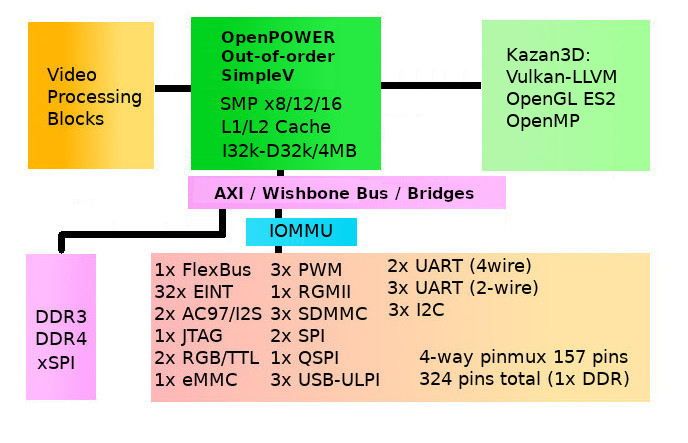
\includegraphics[width=0.9\textwidth]{shakti_libre_soc.jpg}
\end{center}

}

\frame{\frametitle{Summary}

 \begin{itemize}
   \item Goal is to create a mass-volume low-power embedded SoC suitable
         for use in netbooks, chromebooks, tablets, smartphones, IoT SBCs.
   \item No way we could implement a project of this magnitude without
         nmigen (being able to use python OO to  HDL)
   \item Collaboration with OpenPOWER Foundation and Members absolutely
         essential. No short-cuts.  Standards to be developed and ratified
         so that everyone benefits.
   \item Riding the wave of huge stability of OpenPOWER ecosystem
   \item Greatly simplified open 3D and Video drivers reduces product
         development costs for customers
   \item It also happens to be fascinating, deeply rewarding technically
         challenging, and funded by NLnet
         
  \end{itemize}
}


\frame{
  \begin{center}
    {\Huge The end\vspace{12pt}\\
		   Thank you\vspace{12pt}\\
		   Questions?\vspace{12pt}
	}
  \end{center}
  
  \begin{itemize}
	\item Discussion: http://lists.libre-soc.org
	\item OFTC IRC \#libre-soc
	\item http://libre-soc.org/
	\item http://nlnet.nl/PET
	\item https://libre-soc.org/nlnet/\#faq
  \end{itemize}
}

\end{document}
